%% LaTeX2e class for student theses
%% sections/evaluation.tex
%% 
%% Karlsruhe Institute of Technology
%% Institute for Program Structures and Data Organization
%% Chair for Software Design and Quality (SDQ)
%%
%% Dr.-Ing. Erik Burger
%% burger@kit.edu
%%
%% Version 1.3.2, 2017-08-01

\chapter{Evaluation}
\label{ch:Evaluation}

In this section, we introduce the evaluation of our approach. We divided our evaluation into levels. In the first level, we evaluate the adaptive instrumentation. In the second level, we evaluate the monitoring information that we created to make sure that we’ve created the right monitoring information. In the third level, we evaluate our approach in term o reducing the monitoring overhead. \\
In the following we defined the goals (G) and research questions (Q) for our evaluation:

\begin{itemize}[label={}, leftmargin=*]
\item G1: Adaptive Instrumentation
  \begin{itemize}[label={}]
  \item Q1.1: Is our instrumentation of the source code incremental?
      \begin{itemize}[label={}]
      \item M1.1.1: difference between the probes in the instrumentation model and the generated probes in the            
                    instrumented source code.  
      \end{itemize}
   \item Q1.2: did we generate the right monitoring information?
        \begin{itemize}[label={}]
             \item M1.2.1: Number of acceptances of our monitoring information from performance model parameters  
	                       estimation approach.
      \end{itemize}
  \end{itemize}
\item G2: Adaptive Monitoring
   \begin{itemize}[label={}]
   \item Q2.1: How much monitoring overhead could we reduce?
       \begin{itemize}[label={}]
        \item M2.1.1: number of generated monitoring records. 
       \end{itemize}
   \end{itemize}
\end{itemize}



\section{Case Study}
\label{sec:Case Study}
In order to evaluate our approach, we performed a case study that is represented by the component diagram in Figure \ref{fig:case_study}. We created two Java interfaces and we implemented them. The first interface \textit{ISearchingAlgo} contains two functions. The service \textit{sequentianSearch}, which receives an Array of integers and a value of type integer, it returns True if the given value exists in the given array. This service is based on the sequential searching algorithm. The second service \textit{binarySearch} perform receives also an Array of integers and an integer value, it must then tell us if the given could be found in the given array. The service \textit{binarySearch} is implemented based on the binary searching algorithm. The binary searching algorithm is more efficient then the sequential searching algorithm, we choose these algorithms to provide the possibility of having different response times and service calls parameters. 

The second interface \textit{GuiSearchingAlgo} provides also two services and requires services from the interface \textit{ISearchingAlgo}. The service \textit{guiSeuentialSearch} receives two arrays of integers, the first array represents the array in which we want to perform the searching, the second array represent the values we want to search for. This service iterates over the  array of values that we want to search for and calls the service \textit{sequentialSeach} from the interface \textit{ISearchingAlgo}, which tells if the current searched value could be found. Figure 2 shows the corresponding SEFF of the \textit{guiSequentialSearch} service. The service \textit{guiBinarySearch} in the interface \textit{GuiSearchingAlgo} does the same thing as the service \textit{guiSequentialSearch} but it calls the service \textit{binarySearch} instead of \textit{sequentialSeach} service. 

\begin{figure}[h]
\centering
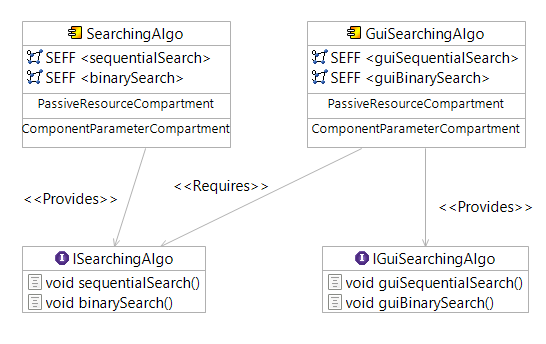
\includegraphics[width=0.9\textwidth]{figures/case_study}
\caption{Component diagram of our case study}
\label{fig:case_study}
\end{figure}

\section{Adaptive Instrumentation}
\label{sec:Adaptive Instrumentation}
In this section, we use our case study to evaluate the incremental instrumentation and the monitoring information types. We evaluate the incremental instrumentation to make sure that we could instrument the source code incrementally in our approach. We evaluate the monitoring information types to make sure that we've generated the right information that can be used by performance model parameters estimation approaches. 

\subsection{Incremental Instrumentation}
\label{sec:Incremental Instrumentation}
In the first level of our evaluation, we evaluate the incremental instrumentation of our approach. As a metric for this evaluation, we decided to compute the difference between the probes in the instrumentation model and the monitoring probes in the instrumented source code in each iteration. The reason we used this metric is because of the incremental generation of probes in our instrumentation model. That means, in each iteration, we collect only the probes of the changed parts of the sour code and save them in the instrumentation model. Moreover, if we instrumented the source code incrementally, all the probes in the instrumented source code must be found in the instrumentation model. That means also that the difference between the probes in the logged monitoring information and in the instrumentation model must be empty. However, if this difference is not empty, that means, there exist probes in the instrumented source code, even though they do exist in the instrumentation model. That implied that the instrumentation has been not done incrementally.

In order to return the probes in the instrumented source code, we run it to receive the monitoring records. Each monitoring record corresponds to a monitoring probe in the source code. Moreover, monitoring records are can be identified via the id of their monitoring probes. Therefore, we can use the monitoring records after the execution of the instrumented source code to extract the monitoring probes in the source code. 

Moreover, the monitoring probes in our instrumentation model are saved via their ids. Furthermore, since the monitoring records have the same id as their monitoring probes, we can then compute the difference between the existing ids of the probes in the instrumentation model and ids of the monitoring records in the monitoring information. 

As mentioned above, in order to evaluate the incremental instrumentation, we calculate the difference between the probes in the monitoring information and in the instrumented source code. Therefore, we created two iterations Figure \ref{fig:incremental_instr_eva}. In the first iteration, we changed the source code of our case study by implementing the services \textit{sequentialSearch} and \textit{guiSquentialSearch}. During the source code changes, we collected the probes of the changed parts of the source code, then we instrument the source code based on these probes. Then, we executed the instrumented source code to generate the monitoring information. 

In the second iteration, we changed the services \textit{binarySearch} and \textit{guiBinarySearch}. Then, we followed the same steps in the first iteration to generate the monitoring information for the second iteration. 


Figure \ref{fig:incremental_instr_eva}, shows that the difference between the probes in the instrumented source code and the probes in the instrumentation model is empty in the first and in the second iteration, which means our instrumentation has executed incrementally. \\ 


\begin{figure}[h]
\centering
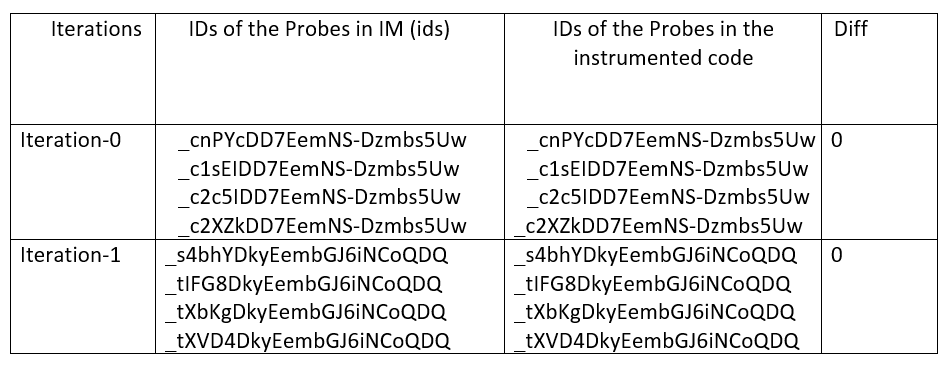
\includegraphics[width=0.9\textwidth]{figures/incremental_instr_eva}
\caption{difference between the probes in the instrumentation mode and in the monitoring, information is empty in the first and the second iteration, which means our instrumentation for the case study has been done incrementally}
\label{fig:incremental_instr_eva}
\end{figure}



\subsection{Monitoring Information} 
\label{sec:Monitoring Information}
In the second level of our evaluation, we evaluate the monitoring information that we log using our incremental instrumentation. The source code that we instrument has to provide monitoring information that can be used to estimate parameters for the Palladio performance model. 

Our monitoring information is defined in records (Section records), which are four types, namely response time record, loop record, branch record, and service call record. 

In order to make sure that we generate the right records, we've instrumented our case study and executed the instrumented source code to generate the monitoring records for all types of records that we defined in our approach. Then, we used our monitoring records and the performance model parameters approach of Jägers [ref] to estimate the parameters for the Palladio Performance Model.

Figure 2 shows the SEFF that corresponds to the service \textit{guiSequetialSearch}. The estimated parameters of this model have been done based on our monitoring records. Moreover, the case study contains all the record types that we defined, which gives us the possibility make sure that all the records that we defined can be used in the palladio performance model parameters estimation.


\begin{figure}[h]
\centering
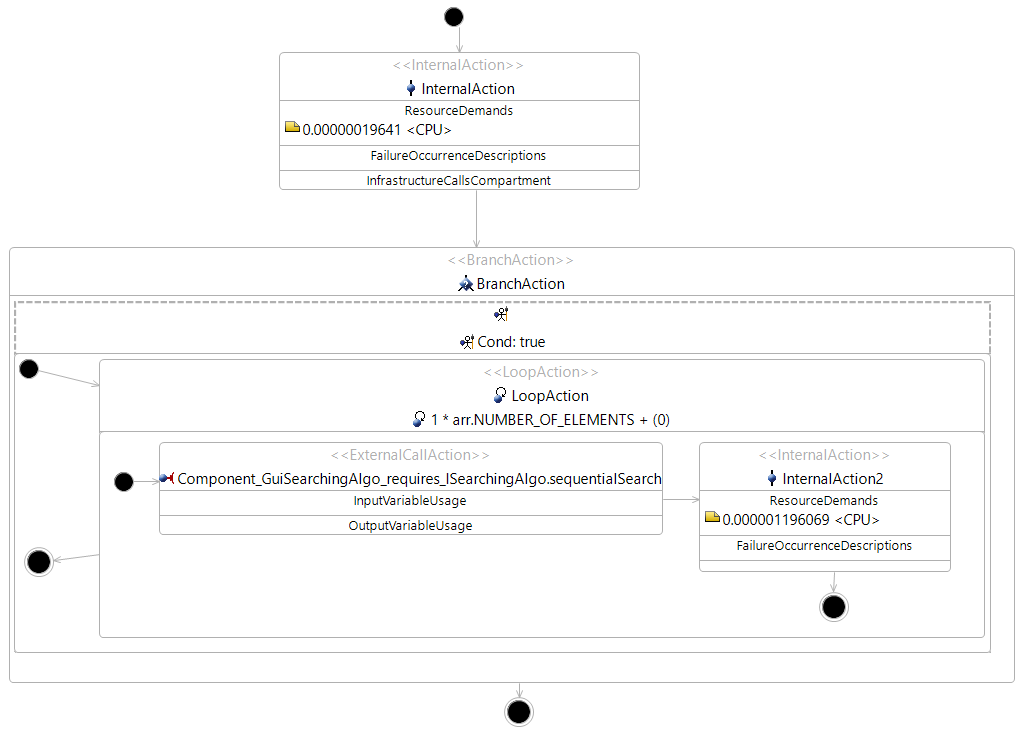
\includegraphics[width=0.9\textwidth]{figures/records_evaluation}
\caption{shows the SEFF of the service \textit{guiSequentialSearch} and its estimated parameters based on our records that received from monitoring this service}
\label{fig:guiSequentialSearch_seff}
\end{figure}


\section{Adaptive Monitoring}
\label{sec:Adaptive Monitoring}
In the third level of our evaluation, we answer the question, how much monitoring overhead can we reduce using our approach. 

Our experiment is based on the instrumentation of the source code in (Section incremental instrumentation). After we run the instrumented source code in the iteration-0, we counted 6700 records for one load test. For the monitoring of the instrumented source code in the iteration-1, we counted 6700 records for one load test. 

In we instrument completely the source code in the iteration-1, we count 13400 records for one load test. If we instrument incrementally the source code in the iteration-1, we receive 6700 records, which is about 50\% the amount we count if we did not instrument the source code incrementally.







